% !TEX encoding = UTF-8 Unicode

%% Document Details
\newcommand{\docTitle}{The Spidergon Network-on-Chip}
\newcommand{\docAuthor}{Andrew Fecheyr Lippens}
\newcommand{\docDate}{\today}
\newcommand{\docSubject}{Redes en Chip}

% !TEX encoding = UTF-8 Unicode

\documentclass[12pt]{article}
\usepackage[utf8]{inputenc}
\usepackage[english]{babel}
\usepackage[pdftex]{graphicx}
\usepackage{fancyhdr}
\usepackage{url}
\newcommand{\HRule}{\rule{\linewidth}{0.5mm}}
\usepackage{geometry}
\usepackage[font=small,format=plain,labelfont=bf,up,margin=1cm]{caption}
\usepackage[pdftex,bookmarks=true,pdfborder={0 0 0},pdfauthor={\docAuthor},pdftitle={\docTitle},pdfsubject={\docSubject}]{hyperref}
\geometry{a4paper}

%% Set the document details
\title{\docTitle}
\author{\docAuthor}
\date{\docDate}

%% unbreakable words
\hyphenation{multi-core}

%%% BEGIN DOCUMENT
\begin{document}
\begin{titlepage}
\begin{center}
 
% Upper part of the page

\includegraphics[width=0.50\textwidth]{../shared/figures/logoUPV.pdf}\\[1cm]
\textsc{\LARGE Universidad Polit\'ecnica de Valencia}\\[1.4cm]
\textsc{\Large \docSubject}\\[1.4cm]
 
 
% Title
\HRule \\[0.4cm]
{ \huge \bfseries \docTitle}
\HRule \\[1.4cm]
 
% Author and supervisor
\begin{flushleft} \large
\emph{Author:}\\
\docAuthor
\end{flushleft}

\vfill
 
% Bottom of the page
{\large \docDate}
 
\end{center}
\end{titlepage}

\begin{abstract}
	\todo[write an abstract]
\end{abstract}

\setcounter{tocdepth}{2}
\begin{tableofcontents}
\end{tableofcontents}

%%% Add some whitespace between paragraphs
\addtolength{\parskip}{0.5\baselineskip}

\newpage

\section{Introduction}\label{C:intro}

A network-on-chip or NoC has become one of the key components in digital chips. 
As the number of components and transistors per chip grows continuously, most chips have become multi-core. 
These chips consist of a number of separate cores, often with fixed-function accelerators, memory arrays and input/output units.
		
Historically buses or crossbar switches were used to connect the functional components of a chip. 
Above four cores, however, the limited bandwidth of a bus becomes a major limitation, and above 8 or 16 cores, crossbar switches become very expensive. 
Only a NoC provides the scalability needed for emerging multicore chips. 
The NoC bounds the performance potential of these chips and accounts for a substantial fraction of the power and area consumption.

\todo[introduce Spidergon]

\section{Background}\label{C:background}

\subsection{Technical Terms}\label{S:terms}
	
This paper uses technical terms from the domain of computer networks. 
Some of them are explained here to help the reader.

\begin{description}

\item[System on Chip (SoC)] 
	
refers to the integration of all components of a computer or electronic system into a single integrated circuit (chip) \cite{wikiSoC}. SoCs are often used in space and power constrained devices.
	
\item[A Network on Chip (NoC)] 

is a packet-switched on-chip micronetwork. 
It is the natural evolution of traditional circuit-switched bus solutions. 
	
\item[An Interconnect Processing Unit (IPU)] 
	
is a configurable and extensible communication component that implements system services and core communication. 
It is essentially an on-chip communication network with hardware and software elements which jointly implement key functions of different SoC programming models through a set of communication and synchronization primitives and provide low-level platform services to enable advanced features in modern heterogeneous multi-core SoCs.\cite{coppola2008design}

\item[A Chip multiprocessor (CMP)] 

is a multi-core processor in which the distinct cores are integrated onto a single integrated circuit die.

\item[IP block:] 
	
In electronic design a semiconductor intellectual property core or IP block is a reusable unit of logic, cell, or chip layout design that is the intellectual property of one party. 
They are often used as building blocks in SoC designs.

\end{description}

\subsection{Bus vs. Network-on-Chip}\label{S:busvsnoc}

SoC communication has traditionally been done using on-chip busses. 
A diagram of an early bus architecture is depicted on figure \ref{fig:soc_bus}. 
This allowed designers of early SoCs to select IP blocks, place them onto the silicon, and connect them together with a standard on-chip bus.

	\begin{figure}[ht]
	\centering
		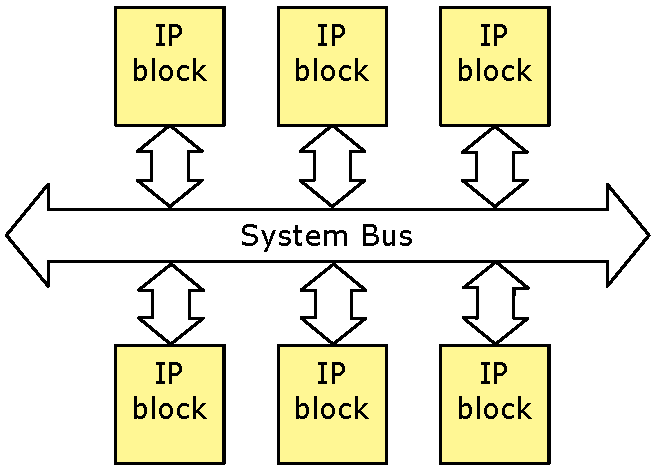
\includegraphics[width=0.50\textwidth]{soc_bus}
		\caption{Early SoC structure based on a single shared bus}
		\label{fig:soc_bus}
	\end{figure} 

Buses are well understood and have been successfully implemented in many complex SoCs focusing on both application-based and processor-specific features, thus providing compatibility with most available IP and processor cores, and SoC communication requirements. Examples of more modern on-chip buses include ST Microelectronics' STBus~\cite{scandurra2002stbus}, ARM's AMBA AHB and IBM's Core-connect \cite{ryu2001comparison}.

However, buses do not scale well. With the rapid rise in the number of blocks to be connected and the
increase in performance demands, today's SoCs cannot be built around a single bus. Instead, complex hierarchies of buses are sometimes used, with sophisticated protocols and multiple bridges between them.
Communication between two remote blocks can go via several buses, and every section of every path must be carefully verified \cite{furber2005future}. 

Moreover, the increase in the number of connected IP and processor cores causes the bus to become a communication bottleneck due to sharing of aggregate bandwidth by all attached units, and worsens arbiter delay, thus introducing variation, limiting scalability and making the arbiter instance-specific. Additional concerns regarding reachable clock frequency and time closure arise, since every bus transaction involves all connected cores and unnecessarily consumes significant power~\cite{coppola2008design}.


	\begin{figure}[ht]
	\centering
		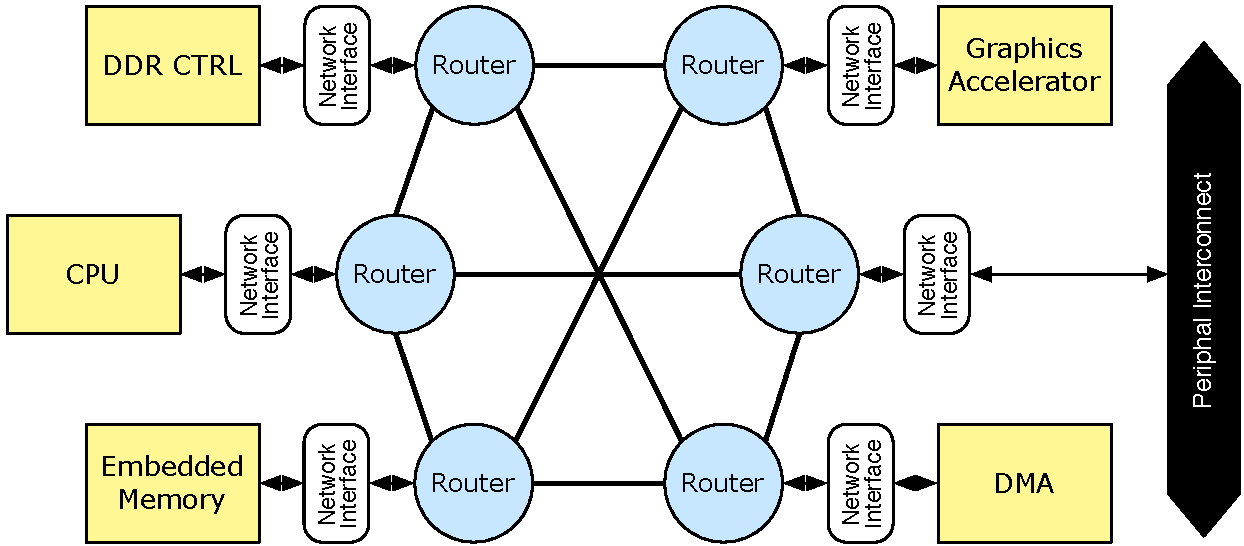
\includegraphics[width=1.0\textwidth]{soc_noc}
		\caption{SoC equipped with a Network-on-Chip}
		\label{fig:soc_noc}
	\end{figure} 

\section{Spidergon STNoC}\label{C:stnoc}

As a first attempt at designing a configurable IPU, Spidergon STNoC IPU technology consists of a flexible, pseudo-regular on-chip communication network implementing a set of customizable low-level platform services and a set of communication primitives.

The Spidergon STNoC IPU is a software programmable on-chip communication network that enables system designers to extend communication primitives. 
These communication primitive extensions are then automatically synthesized, placed, and routed into the Spidergon STNoC communication network. 
The communication network leverages graph properties of the Spider- gon regular topology discussed, while matching heterogeneity of Multicore SoCs through software programmability concepts, application-specific hardware configurability and extensibility.

Existing NoC architectures are either based on a fixed regular network topology, or they are topology-independent, i.e. they can be customized to a particular application-specific communication graph. 
The Spidergon STNoC topology fills the gap between these two approaches, trading off regularity with customizability; for this reason, it is sometimes called a pseudo-regular topology\cite{coppola2008design}. 
Using this concept, NoC topology becomes an architectural parameter that can be configured depending on the communication patterns exhibited by the application. 
Moreover, in order to address Multicore application requirements for feature-rich devices, e.g. speech processing, video, GPS, security, and mobility, Spidergon STNoC technology provides a set of low-level platform services. 
The most important services defined in Spidergon STNoC are security, power management, and QoS. 
These services can be instantiated depending on the real target application and may be augmented by customer-specified services.

\subsection{Spidergon Topology}\label{S:topology}

The Spidergon topology provides an interesting price/performance trade-off for SoC devices. 
In the Spidergon topology, all of the IP blocks are arranged in a ring where each IP block is connected to its clockwise and its counter-clockwise neighbour and directly to its diagonal counterpart in the network. 
This allows the routing algorithm to minimise the number of nodes that a data packet has to traverse before reaching its destination. 
A particularly important advantage is that the functional diagram (shown below on the left of figure \ref{fig:topology} for a network of 16 nodes) corresponds to a simple planar implementation (shown on the right side of figure \ref{fig:topology}) in which the wiring only needs to cross itself at one point. This is a key benefit in delivering high price/performance~\cite{STMicroelectronics2005}.

	\begin{figure}[ht]
	\centering
		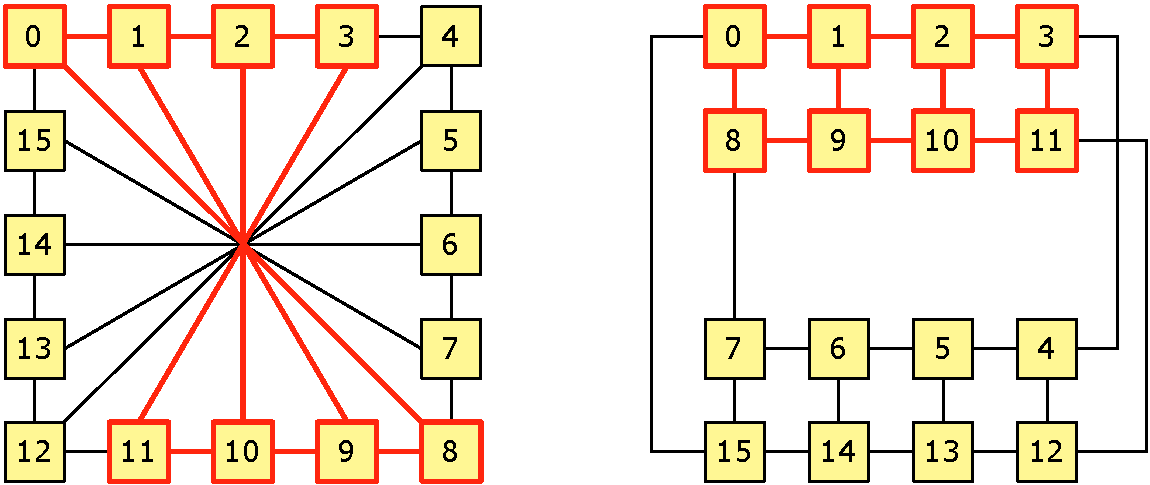
\includegraphics[width=0.75\textwidth]{topology3}
		\caption{Equivalent representations of the Spidergon topology for ${N}$ = 16}
		\label{fig:topology}
	\end{figure}

Topologies with increased connectivity, such as 2D mesh, provide very good theoretical metrics, but in most cases, these features cannot be fully exploited due to the nature of communication traffic in Multicore SoC applications. 
On the other hand, simple topologies, such as rings, are cost-effective in terms of manufacturing cost, but deliver relatively poor performance, especially as the number of connected cores increases. Spidergon tries to strike a balance in this tradeoff. 

Compared to complex topologies, Spidergon offers a small number of links and simple implementation. For current, realistic NoC configurations with up to 60 nodes, the proposed Spidergon graph has a smaller number of edges and a competitive network diameter with respect to fat-tree or 2D mesh topologies.

Figure \ref{fig:different_topologies} illustrates different families of topologies supported by the Spidergon STNoC. 
These topologies are essentially degree 2 or 3 Spidergon subgraphs that range from rings and simple spanning trees to irregular chordal rings. 
Depending on application traffic requirements and especially mapping of master and slave agents, connection paths can be removed if never used and cross connections customized to provide shortcuts between any pair of nodes in the ring.

	\begin{figure}[ht]
	\centering
		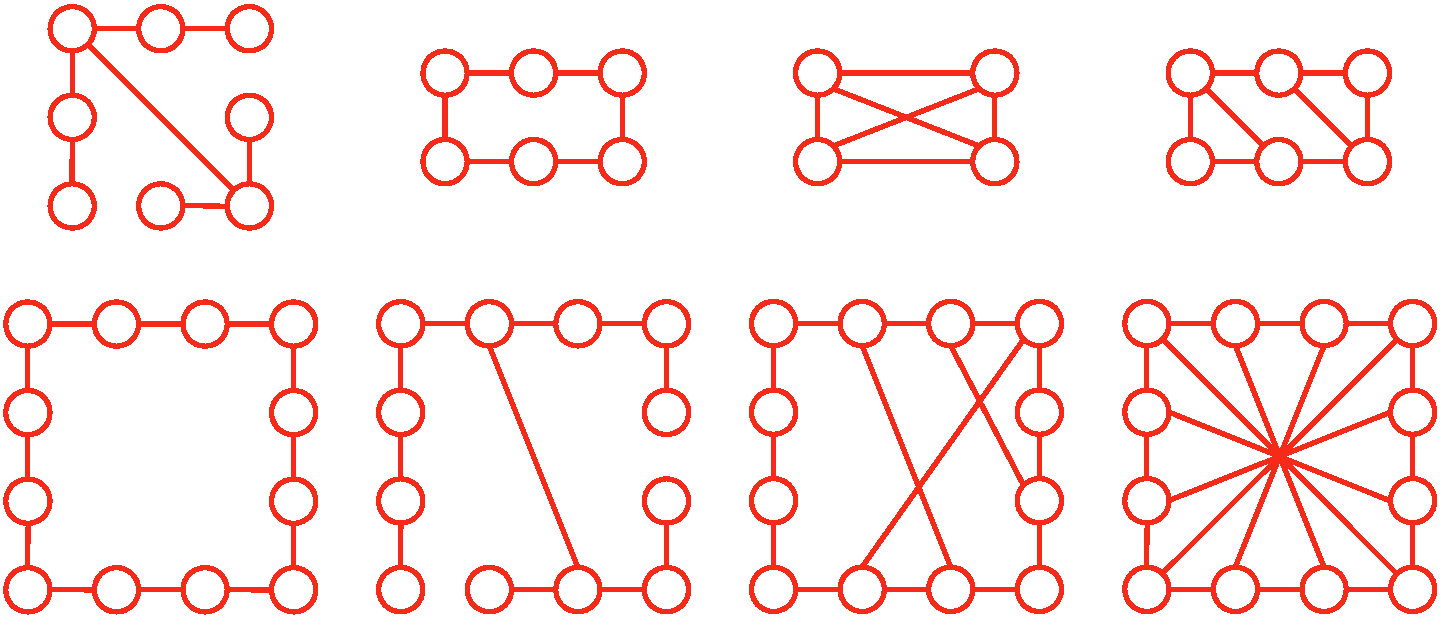
\includegraphics[width=0.75\textwidth]{different_topologies}
		\caption{Different topologies supported by Spidergon STNoC}
		\label{fig:different_topologies}
	\end{figure}

\subsection{Topology Comparison}\label{S:metrics}

Each NoC topology offers a different set of tradeoffs in terms of metrics, such as:
\begin{itemize}
\item Vertex symmetry, which affects routing or scheduling cost and performance,
\item Network degree, which affects the operating frequency and the complexity of the routers,
\item Network extendibility, which should be as low as possible to maximize flexibility in Multicore designs, and 
\item Average distance between nodes.
\end{itemize}

Table \ref{tab:metrics} presents a summary of static topological metrics for three typical NoC topologies: Ring, Spidergon and ${m \times n}$ Mesh.

\begin{table}[ht]
\begin{center}
\begin{tabular}{|p{1.1in}|p{1.1in}|p{1.4in}|p{1.3in}|}
	\hline
	\textbf{Property} & \textbf{Ring} & \textbf{Spidergon} & \textbf{2D ${n \times m}$ Mesh} \\ \hline 
	\textbf{Symmetry} & both & vertex & no \\ \hline
	\textbf{Degree} & 2 & 3 & 4 \\ \hline
	\textbf{Links} & ${2N}$ &  ${3N}$ & ${4mn - 2m - 2n}$  \\ \hline
	\textbf{Extendibility} & 1 & 2 & min${(m,n) \geq 2 }$ \\ \hline
	\textbf{Node \mbox{connectivity}} & 2 & 3 & 2 \\ \hline
	\textbf{Diameter} &${N/2}$ & ${N/4}$ & ${m + n - 2}$ \\ \hline
	\textbf{Average \mbox{distance}} 
		& if ${N}$ even: \par
			\hspace{2mm} ${N/4}$ \par 
		if ${N}$ odd: \par
			\hspace{2mm} ${(N^2-1)/4N}$
		& if ${N = 4n}$: \par 
			\hspace{2mm} ${(2n^2 + 2n - 1)/N}$ 
		if ${N = 4n +2}$: \par 
			\hspace{2mm} ${(2n^2 + 4n + 1)/N}$
		& \vspace{1mm} $\frac{\displaystyle(m + n)(mn - 1)}{\displaystyle3mn}$\\ \hline
	\textbf{Bisection width} & 4 
		& if ${N = 4n}$: 8 \par
		if ${N = 4n +2}$: 10
		&  if max(${m}$,${n}$) even: \par
			\hspace{2mm} 2min(${m}$,${n}$)  \par 
		if max(${m}$,${n}$) odd: \par
			\hspace{2mm} 2min(${m}$,${n}$) + 2 \\ \hline
\end{tabular}
\caption{Theoretical metrics for different topologies}\label{tab:metrics}
\end{center}
\end{table}

The data shows that for ${N < 60}$, the Spidergon topology despite its constant bisection is very competitive. 
Due to its higher connectivity, the Spidergon topology always outperforms Rings in terms of diameter and average distance. Spidergon also competes favorably or outperforms 2D Mesh, although outcomes depend on network size. 
In fact, while Spidergon properties scale linearly with the network size, 2D Mesh behavior is quite irregular. 
This irregularity is a severe bottleneck in Multicore SoC design, since it complicates design space exploration in terms of cost-performance tradeoffs. For example, a 22 node 2D mesh has smaller diameters and average distance metrics than a 24 node 2D mesh.

\subsection{Switching Strategy}\label{S:switching}

The switching strategy refers to how a packet traverses the route. 
More specifically, the switching technique determines how a message is fragmented and transmitted from an input of the on-chip network to an output resource by defining how channels and possible buffers along the path are allocated. 
There are four types of switching techniques:
\begin{itemize}
\item Circuit switching,
\item Store-and-forward,
\item Wormhole, and 
\item Virtual Cut-through.
\end{itemize}

Spidergon STNoC adopts wormhole routing, which is nowadays commonly used in NoC design. 
Due to this switching technique, the Spidergon STNoC router has a simple architecture, occupies a small area, and is extremely fast in terms of operating frequency.

\section{Evaluation}\label{C:evaluation}
	\todo[look for good evaluation resources]

\section{Conclusion}\label{S:conclusion}
	\todo[write a conclusion]

\bibliographystyle{plain}
\bibliography{spidergon}

\end{document}

